% 
% Licensed to the Apache Software Foundation (ASF) under one
% or more contributor license agreements.  See the NOTICE file
% distributed with this work for additional information
% regarding copyright ownership.  The ASF licenses this file
% to you under the Apache License, Version 2.0 (the
% "License"); you may not use this file except in compliance
% with the License.  You may obtain a copy of the License at
% 
%   http://www.apache.org/licenses/LICENSE-2.0
% 
% Unless required by applicable law or agreed to in writing,
% software distributed under the License is distributed on an
% "AS IS" BASIS, WITHOUT WARRANTIES OR CONDITIONS OF ANY
% KIND, either express or implied.  See the License for the
% specific language governing permissions and limitations
% under the License.
% 
\chapter{Building and Testing Jobs}

\section{Overview}

A DUCC job consists of two process types, a Job Driver process and one or more
Job Processes. These processes are connected together via UIMA-AS.
The Job Driver process wraps the job's Collection Reader (CR). The CR
function is to define the collection of Work Items to be processed.
The Collection Reader returns a small CAS for each Work Item containing a
reference to the Work Item data
The Job Driver uses the UIMA-AS client API to send Work Item CASes 
to the job's input queue. Job Processes containing the analytic pipeline are deployed
as UIMA-AS services and comsume CASes from the job input queue.

A basic job's analytic pipeline consists of an Aggregate Analysis Engine comprised by
the user specified CAS Multiplier (CM), Analysis Engine (AE) and CAS
Consumer (CC) components, along with a built-in DUCC Flow Controller.
The Work Item CAS is typically sent only to the CM and returned by
the Job Process when all child CASes produced by the CM have completed
processing; optionally the CR can configure Work Item CAS flow to go to the CC 
or to the AE \& CC to complete all processing for that Work Item.

	\begin{description}
	    \item[Note:] Although the Job Driver will receive back the Work Item CAS, 
	    there is no provision for any user code to receive the CAS. Therefore a
		Job Process typically adds no results to a Work Item CAS.
	\end{description}

   \subsection{Basic Job Process Threading Model}
   In addition to the pipeline definition of explicitly named CM, AE and CC components, the job
   specification also includes the number of pipeline threads to run in each
   Job Process (using the job specification parameter: process\_thread\_count).
   Each pipeline thread receives Work Items independently.

   DUCC creates an aggreate descriptor for the pipeline, and then creates a
   Deployment Descriptor for the Job Process which specifying the number
   of synchronous pipelines.
   
   \subsection{Alternate Pipeline Threading Model}
   Alternately a Job Process can be fully specified by a user submitted UIMA-AS
   Deployment Descriptor. Thus any UIMA-AS service deployment can be used as a
   Job Process. Here the parameter process\_thread\_count just defines
   how many Work Items CASes will be sent to each Job Process concurrently.
   
	\begin{description}
	    \item[Note:] In general a UIMA-AS service may be configured to
	    return child CASes; although child CASes returned from a Job Process will be
	    ignored by the Job Driver, there may be significant overhead in wasted
	    serialization and I/O.
	\end{description}

   \subsection{Overriding UIMA Configuration Parameters}
   UIMA configuration parameters in the CR, CM, AE or CC components can be overriden using
   job specification parameters: driver\_descriptor\_CR\_overrides, process\_descriptor\_CM\_overrides,
   process\_descriptor\_AE\_overrides and process\_descriptor\_CC\_overrides, respectively.

   Another approach is to use the {\em External Configuration Parameter Overrides} mechanism
   in core UIMA. External overrides is the only approach available for jobs submitted with
   a Deployment Descriptor.


\section{Collection Segmentation and Artifact Extraction}

UIMA is built around artifact processing. A classic UIMA pipeline starts with
a Collection Reader (CR) that defines collection seqmentation, extracts the artifacts
to be analyzed and puts them into the CASes to be delivered to subsequent analytic components. 
A CR designed for a specific data collection is highly reusable
for many different analytic scenarios.

A single CR supplying artifacts to a large number of analysis pipelines 
would be a bottleneck. Not only would artifact data need to be transported twice across
the compute cluster, but analysis results would be uselessly returned to the Job Driver.
To solve both of these problems, in a DUCC job the CR only sends a reference
to the artifacts in the Work Item CAS, and artifact data is read directly by the analysis pipeline.

In DUCC collection processing the role of collection segmentation is
implemented by the CR run in the Job Driver, while
artifact extraction and CAS initialization are implemented in the Cas Multiplier
(CM) run in the Job Process. The combination of a CR and associated CM 
should be highly reusable. 

\begin{description}
    \item[Note:] In many cases it is useful to reference multiple artifacts in a
      Work Item CAS. Both DUCC sample applications described below exhibit this design.
\end{description}

\section{CAS Consumer Changes for DUCC}

CAS Consumers in a UIMA pipeline may require changes for scale out into DUCC
jobs, to avoid scale out bottlenecks, to preserve collection level
processing, or to flush results at end-of-work-item processing.
   
	\begin{description}
	    \item[Federated ouput:] Scaled out DUCC jobs distribute artifact processing
	    to multiple pipeline instances. All instances of a CAS Consumer should have
	    independent access to the output target (filesystem, service, database, etc.).
	    \item[Singleton processing:] Collection level processing
	    requiring that all results go to a singleton process would usually be done as a 
            follow-on job, allowing
	    incremental progress; Job Process errors due to data-dependent analysis bugs
	    can often be fixed without invalidating completed Work Items, 
            enabling a restarted job to utilize the progress made by
	    previous job runs.
	    \item[Flushing cached data:] In some scenarios each Work Item delivered to a
	    pipeline can be considered an independent collection. If a CAS Consumer
	    caches data which needs to be flushed after processing the
	    last artifact for a Work Item, the Work Item CAS can be routed to the CAS Consumer after
	    the last artifact CAS is processed and used to trigger cache flushing.
	\end{description}


\section{Job Development for an Existing Pipeline Design}

Assuming that an existing job input-output design (CR, CM, CC) is to be reused, job
development is focussed on the Analysis Engine (AE) to be plugged in. Before deploying a new
AE in a multithreaded Job Process it is best to run it single threaded
(process\_thread\_count=1) to separate basic logic errors from threading
problems.

To debug a Job Process with eclipse, first create a debug configuration for a
"remote java application", specifying "Connection Type = Socket Listen" on some
free port P. Start the debug configuration and confirm it is listening on the specified port.
Then add to the job specification
process\_debug=port, where port is the value P used in the running debug configuration.

When the process\_debug parameter is specified, DUCC will only run a single Job Process
that will connect back to the eclipse debug configuration.


\section{Job Development for a New Pipeline Design}

A DUCC job is a UIMA application comprised of user code broken into a Collection
Reader running in the Job Driver and an Agreggate Analysis Engine (analysis pipeline) running in one 
or more Job Processes. Each Job Process may run multiple instances of the pipeline, each in a different
thread. The major components of the basic Job Process application are as follows:

\begin{itemize}
  \item User Collection reader - segments the input collection in to Work Items
  \item User CAS Multiplier - inputs a Work Item and segments it into artifacts (CASes)
  \item User Analysis Engine - processes the CASes
  \item User CAS Consumer - outputs results for each Work Item
  \item DUCC built-in Flow Controller - routes Work Item CASes to the CM and optionally to the CC or AE \& CC.
\end{itemize}

It is good if the CR+CM+CC combination can be reused for a broad range of AE.

\subsection{Collection Reader (CR) Characteristics}
A DUCC Job CR sends Work Item CASes to the Job Processes. These CASes contain references to the data
to be read by the Job Processes. Typically the CR Type System will be very small; in the DUCC sample
applications the CR Type System only contains the Workitem Feature Structure described below.

\begin{description}
    \item[Note:] It is important not to include the analytic Type System in the CR. These Type Systems 
can be quite large and will significantly increase the size of each Work Item CAS. 
The Job Driver process maintains a CAS pool which must be as large
as the total number of processing threads active in a job. 
\end{description}

\subsection{DUCC built-in Flow Controller}
\begin{sloppypar}
This flow controller provides separate flows for Work Item CASes and for CASes produced by the CM and/or AE.
Its behavior is controlled by the existence of a CM component, and then further specified by the
org.apache.uima.ducc.Workitem feature structure in the Work Item CAS.
\end{sloppypar}

When no CM is defined the Work Item CAS is simply delivered to the AE, and then to the CC if defined. 
Any CASes created by the AE will be routed to the CC.

With a defined CM, the Work Item CAS is delivered only to the CM, and then returned from the JP when processing
of all child CASes created by the CM and AE has completed. Work Item CAS flow can be further refined by the CR by
creating a org.apache.uima.ducc.Workitem feature structure and setting the setSendToLast feature to true,
or by setting the setSendToAll feature to true.

\subsection{Workitem Feature Structure}
In addition to Work Item CAS flow control features, the WorkItem feature structure includes other features that are useful
for a DUCC job application. Here is the complete list of features:

\begin{description}[labelindent=0.5in,leftmargin=0.5in]
  \item[sendToLast] (Boolean) - indicates the Work Item CAS be sent to the CC
  \item[sendToAll] (Boolean) - indicates Work Item CAS be sent to the AE and CC
  \item[inputspec] (String) - reference to Work Item input data
  \item[outputspec] (String) - reference to Work Item output data
  \item[encoding] (String) - useful for reading Work Item input data
  \item[language] (String) - used by the CM for setting document text language
  \item[bytelength] (Integer) - size of Work Item
  \item[blockindex] (Integer) - used if a Work Item is one of multiple pieces of an input resource
  \item[blocksize] (Integer) - used to indicate block size for splitting an input resource
  \item[lastBlock] (Boolean) - indicates this is the last block of an input resource
\end{description}

\subsection{Deployment Descriptor (DD) Jobs}
Job Processes with arbitrary aggregate hierarchy, flow control and threading can be fully specified
via a UIMA AS Deployment Descriptor. DUCC will modify the input queue to use DUCC's private
broker and change the queue name to correspond to the DUCC job ID.

\subsection{Debugging}
It is best to develop and debug the interactions between job application components as one, 
single-threaded UIMA aggregate. DUCC provides an easy way to accomplish this, for both basic
and DD job models, using the all\_in\_one specification parameter.

\begin{description}
    \item[all\_in\_one=local] When set to local, all Job components are run in the same
      single-threaded process, on the same machine as eclipse.
    \item[all\_in\_one=remote] With remote, the single-threaded process is run on a DUCC
      worker machine as a DUCC Managed Reservation. 
\end{description}

To debug an all\_in\_one job with eclipse, first create a debug configuration for a
"remote java application", specifying "Connection Type = Socket Listen" on some
free port P. Start the debug configuration and confirm it is listening on the specified port.
Then, before submitting the all\_in\_one job, add the argument process\_debug=port, 
where port is the value P used in the running debug configuration.


\chapter{Sample Application: Raw Text Processing}

\section{Application Function and Design}
This application expects as input a directory containing one or more flat text files, 
uses paragraph boundaries to segment the text into separate artifacts, 
processes each artifact with the OpenNlpTextAnalyzer, and writes
the results as compressed UIMA CASes packaged in zip files. Paragraph boundaries are defined as
two or more consecutive newline characters.

By default each input file is a Work Item. In order to facilitate processing scale out, 
an optional blocksize parameter can be specified that will be used to break larger 
files into multiple Work Items. Paragraphs that cross block boundaries are processed
in the block where they started. An error is thrown if a paragraph crosses two block
boundaries.

An output zip file is created for each Work Item. The CAS compression format is selectable as
either ZIP compressed XmiCas or UIMA compressed binary form 6 format. When compressed binary
is used, each zip file also contains the full UIMA Type System in ZIP compressed text.
CASes in UIMA compressed binary form 6 format have the same flexibility as an XmiCas in that
they can be deserialized into a CAS with a different, but compatible Type System.

By default any previously completed output files found in the output directory are preserved.
While Work Item processing is in progress the associated output files have "\_temp" appended to their
filenames, and any such incomplete output files are always ignored for subsequent jobs.

\section{Configuration Parameters}
The Collection Reader for this job is the DuccJobTextCR. It has the following configuration
parameters:

\begin{description}[labelindent=0.5in,leftmargin=0.5in]
    \item[InputDirectory] path to directory containing input files.
    \item[OutputDirectory] path to directory for output files.
    \item[IgnorePreviousOutput] (optional) boolean to ignore (overwrite) existing output files.
    \item[Encoding] (optional) character encoding of the input files.
    \item[Language] (optional) language of the input documents, i.e. cas.setDocumentLanguage(language).
    \item[BlockSize] (optional) integer value used to break larger input files into multiple Work Items.
    \item[SendToLast] (optional) boolean to route WorkItem CAS to last pipeline component. Is set to true for this application.
    \item[SendToAll] (optional) boolean to route WorkItem CAS to all pipeline components. Not used in this application.
\end{description}

The CAS Consumer is the DuccCasCC and has the following configuration parameters:

\begin{description}[labelindent=0.5in,leftmargin=0.5in]
  \item[XmiCompressionLevel] (optional) compression value if using ZIP compression. Default is 7, range is 0-9.
  \item[UseBinaryCompression] (optional) boolean to select UIMA binary CAS compression.
\end{description}

\section{Set up a working directory}
For this and the following sample program, create a working directory in a writable filesystem.

Copy to this directory the example job specification files:
\begin{verbatim}
   cp $DUCC_HOME/examples/sampleapps/descriptors/*.job .
\end{verbatim}

Copy a UIMA logger configuration file that suppresses tons of output from OpenNLP:
\begin{verbatim}
   cp $DUCC_HOME/examples/sampleapps/descriptors/ConsoleLogger.properties .
\end{verbatim}

Copy the executable code and resources for the DUCC sample application components:
\begin{verbatim}
   mkdir lib
   cp $DUCC_HOME/lib/uima-ducc/examples/uima-ducc-examples*.jar lib
\end{verbatim}

For reference the source code for DUCC sample applications is in \ducchome/examples/src,
with descriptors in \ducchome/examples/sampleapps/descriptors.

\section{Download and Install OpenNLP}
Download the OpenNLP source distribution from http://opennlp.apache.org and follow the directions in the
{\em UIMA Integration} section of the included documentation to build the UIMA pear file.
Then {\em install} the UIMA pear file in the working directory 
with the {\em runPearInstaller} script and
test it with the UIMA Cas Visual Debugger application.

A small modification of the installed OpenNLP descriptor file
is necessary for DUCC to run the component multithreaded. 
Edit {\em opennlp.uima.OpenNlpTextAnalyzer/desc/OpenNlpTextAnalyzer.xml}
and change the setting for {\em multipleDeploymentAllowed} from false to true.

\section{Get some Input Text}
Choose one or more flat text files in UTF8 format that only use newline characters,
{\em not CR-LF sequences}.
The text should be big enough to see the impact of DUCC job scale out.
We used test data from gutenberg.org at
\begin{verbatim}
   http://www.gutenberg.org/ebooks/search/?sort_order=downloads
\end{verbatim}
downloading 'Plain Text UTF-8' versions of {\em Moby Dick}, {\em War and Peace} and {\em The Complete Works of William Shakespeare} 
as flat text files in
a subdirectory `Books', and removing all 'CR' characters (0xD) as well as extraneous text.

\section{Run the Job}
The job specification, DuccRawTextSpec.job, uses placeholders to reference the working directory
and various operational components located there. As run below the placeholders are resolved
from environmental variables.

The job is submitted from the command line with the following:
\begin{verbatim}
   MyAppDir=$PWD \
   MyInputDir=$PWD/Books \
   MyOutputDir=$PWD/Books.processed \
   $DUCC_HOME/bin/ducc_submit -f DuccRawTextSpec.job
\end{verbatim}

The total size of the three txt files is 9.4Mbytes and with a blocksize of 100000 there are 100 Work Items. Each Job Process is 
configured to run 8 parallel OpenNLP pipelines. To examine the performance of processing with just a single Job Process, 
the job can be submitted as:

\begin{verbatim}
   MyAppDir=$PWD \
   MyInputDir=$PWD/Books \
   MyOutputDir=$PWD/Books.processed \
   $DUCC_HOME/bin/ducc_submit -f DuccRawTextSpec.job \
   --process_deployments_max 1
\end{verbatim}

\section{Job Output}
There will be an output zipfile for every Work Item, with zipfiles containing a compressed CAS for each document (paragraph) 
found in a Work Item. If UseBinaryCompression=true each zipfile will also contain the TypeSystem for the CASes. 
This is needed when deserializing these CASes into a different TypeSystem.

DuccTextCM finds 19245 paragraphs in the three txt files. If the output CASes are stored as 19245 uncompressed XMI files, the total size is 911MB. Using the default ZIP compressed XMI format and packed into 100 Work Item zip files, the total size is 165MB, a 5.5x compression. Using UIMA binary compressed format further reduces total size to 62MB.

This output data will be used as input data for the following CAS input processing sample application.

\section{Job Performance Details}
DUCC captures a number of process performance metrics.
\hyperref[fig:OpenNLP-Process-Measurements]{Figure ~\ref{fig:OpenNLP-Process-Measurements}} shows details on the JD and 
single JP processes. The \%CPU time shown, 728, is lower than the actual because the Job Process was idle 
for some time before it received the first Work Item and also idle between finishing the last Work Item and being shut down.
DUCC shows the JVM spent a total of 58 seconds in 
GC (garbage collection), had no major page faults or page space, and used a max of 2.1GB of RSS.

\begin{figure}[H]
  \centering
  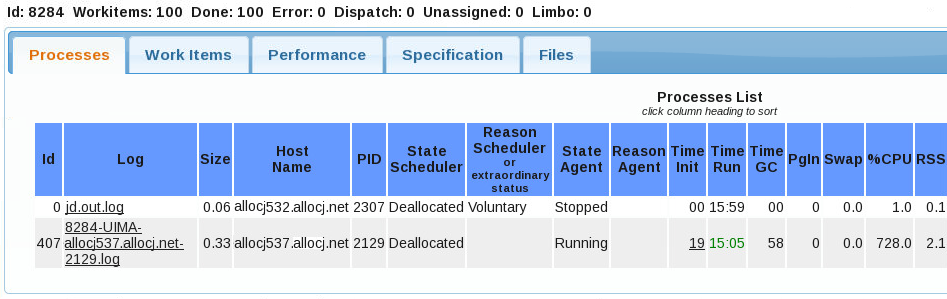
\includegraphics[width=7in]{images/BooksRaw.png}
  \caption{OpenNLP Process Measurements}
  \label{fig:OpenNLP-Process-Measurements}
\end{figure}

On the Performance tab, DUCC shows the breakdown of clock time spent in each primitive UIMA component running in the 
Job Process. See \hyperref[fig:OpenNLP-Process-Breakdown]{Figure ~\ref{fig:OpenNLP-Process-Breakdown}}.
Processing time was dominated by the Parser component at 76.7\%. The time spent compressing and writing out CASes 
was 0.5\%, and the time reading the input text files well below 0.1\%.

\begin{figure}[H]
  \centering
  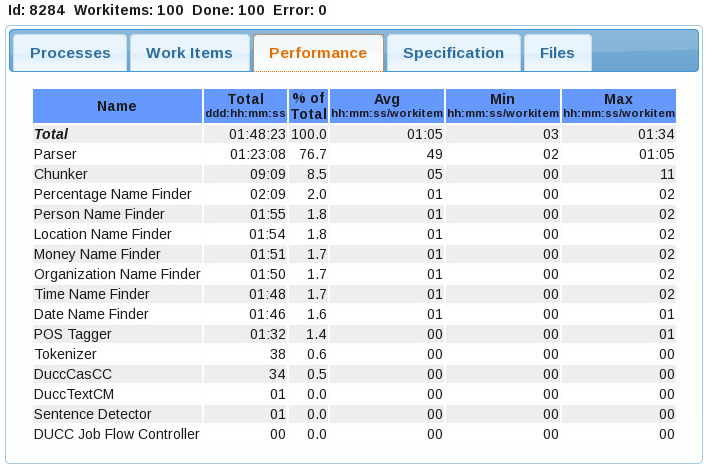
\includegraphics[width=5.5in]{images/BooksRawPerf.png}
  \caption{OpenNLP Process Breakdown}
  \label{fig:OpenNLP-Process-Breakdown}
\end{figure}


\chapter{Sample Application: CAS Input Processing}

\section{Application Function and Design}
The main purpose of this application is to demonstrate the overhead of processing a collection of CASes grouped into 
zipfiles and stored as ZIP compressed XmiCas or with UIMA compressed binary form 6 format.

	\begin{description}
    \item[Note:] This application depends on successful processing of the work in the previous chapter.
	\end{description}

\section{Configuration Parameters}
The Collection Reader for this job is the DuccJobCasCR. It has the following configuration
parameters:

\begin{description}[labelindent=0.5in,leftmargin=0.5in]
    \item[InputSpec] path to directory containing input files (named InputSpec in the hope that more options will be added).
    \item[OutputDirectory] path to directory for output files.
    \item[IgnorePreviousOutput] (optional) boolean to ignore (overwrite) previous output files.
    \item[SendToLast] (optional) boolean to route WorkItem CAS to last pipeline component. Set to true in this application.
    \item[SendToAll] (optional) boolean to route WorkItem CAS to all pipeline components. Not used in this application.
\end{description}


The CAS Consumer is the DuccCasCC and has the following configuration parameters:

\begin{description}[labelindent=0.5in,leftmargin=0.5in]
  \item[XmiCompressionLevel] (optional) compression value if using ZIP compression. Default is 7.
  \item[UseBinaryCompression] (optional) boolean to select UIMA binary CAS compression.
\end{description}

\section{Run the Job}
The job specification, DuccCasInputSpec.job, uses placeholders to reference the working directory
and various operational components located there. As run below the placeholders will be resolved
from environmental variables. 

The job is submitted from the command line with the following:
\begin{verbatim}
   MyAppDir=$PWD \
   MyInputDir=$PWD/Books.processed \ 
   MyOutputDir=$PWD/Books.followon \
   $DUCC_HOME/bin/ducc_submit -f DuccCasInputSpec.job \
   --process_deployments_max 1
\end{verbatim}

\section{Job Performance Details}
\hyperref[fig:CAS-Input-Processing]{Figure ~\ref{fig:CAS-Input-Processing}} shows the component breakdown
using binary CAS compression. Reading and deserializing took 38\% vs the 60\% spent serializing and writing.
Using 8 pipeline threads in one process the 19245 CASes output from the last application were read and 
re-written in 9 seconds.

\begin{figure}[H]
  \centering
  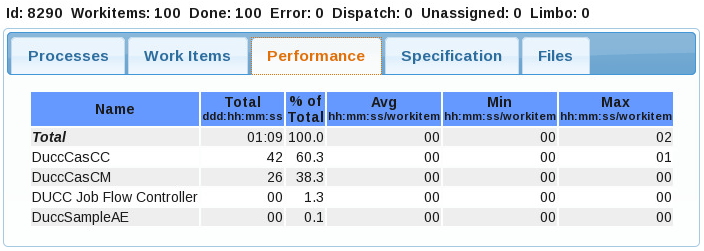
\includegraphics[width=5.5in]{images/BooksCasPerf.png}
  \caption{CAS Input Processing Performacne}
  \label{fig:CAS-Input-Processing}
\end{figure}

\section{Limiting Job Resources}
Although this 8-threaded Job Process was primarily CPU bound doing serialization work, it is possible to become I/O bound 
with enough threads banging on a shared filesystem.
DuccCasInputSpec.job demonstrates how to limit the total number of processing threads to 32 using the combination 
of process\_thread\_count=8 and process\_deployments\_max=4.

I/O vs CPU bottlenecks can be detected using the detailed performance job data reported by DUCC and comparing results
with various levels of scale out.
